\documentclass[border=12pt]{standalone}
\def\pgfsysdriver{pgfsys-dvisvgm.def}
\usepackage[dvisvgm]{xcolor}
\usepackage{xeCJK}
\setCJKmainfont{HaranoAjiGothic-Regular.otf}[BoldFont=HaranoAjiGothic-Bold.otf]
\setCJKsansfont{HaranoAjiGothic-Regular.otf}[BoldFont=HaranoAjiGothic-Bold.otf]
\usepackage{amsmath,amssymb,tikz,lmodern}
\usetikzlibrary{arrows.meta,positioning,calc,fit,backgrounds}
\renewcommand{\familydefault}{\sfdefault}
\definecolor{ink}{HTML}{25322F}
\definecolor{green}{HTML}{246657}
\definecolor{tint}{HTML}{EEF4F0}
\definecolor{soft}{HTML}{C6D2CC}
\definecolor{muted}{HTML}{52615B}
\newif\ifJapanese
\newcommand{\Tx}[2]{\ifJapanese #1\else #2\fi}
\newcommand{\Eff}{\overline{\operatorname{Eff}}}
\newcommand{\heading}[3]{{\color{green}\bfseries #1\quad\Tx{#2}{#3}}\\[5pt]}
% A white rectangle makes the complete citation label clickable, including spaces.
\newcommand{\refurl}[2]{\special{dvisvgm:raw <a xlink:href="#1" target="_blank" rel="noopener noreferrer">}{\setlength{\fboxsep}{0pt}\colorbox{white}{\color{green}\underline{\strut #2}}}\special{dvisvgm:raw </a>}}
\tikzset{
 card/.style={draw=soft,fill=white,rounded corners=2pt,align=left,text=ink,font=\fontsize{10.5}{14}\selectfont,inner xsep=12pt,inner ysep=10pt,text width=14.4cm},
 half/.style={card,text width=6.45cm,minimum height=2.05cm},
 result/.style={card,draw=green,fill=tint,line width=.9pt},
 reason/.style={align=left,text=muted,font=\fontsize{9}{12}\selectfont,inner sep=0pt,text width=12.7cm},
 branchreason/.style={reason,text width=5.95cm},
 edge/.style={-{Stealth[length=2.4mm]},draw=green,line width=1pt},
 wire/.style={draw=green,line width=1pt},
}
% Keep the arrow in a dedicated left gutter; explanations never cover it.
\newcommand{\flow}[3]{
 \coordinate (#2-from) at ($(#1.south)+(-6.9,0)$);
 \coordinate (#2-to) at ($(#2.north)+(-6.9,0)$);
 \draw[edge] (#2-from)--(#2-to);
 \node[reason,anchor=west] (#2-reason) at ($(#2-from)!.5!(#2-to)+(.55,0)$) {#3};
}

\newcommand{\Cite}[2]{\refurl{#1}{#2}}

\Japanesetrue
\begin{document}
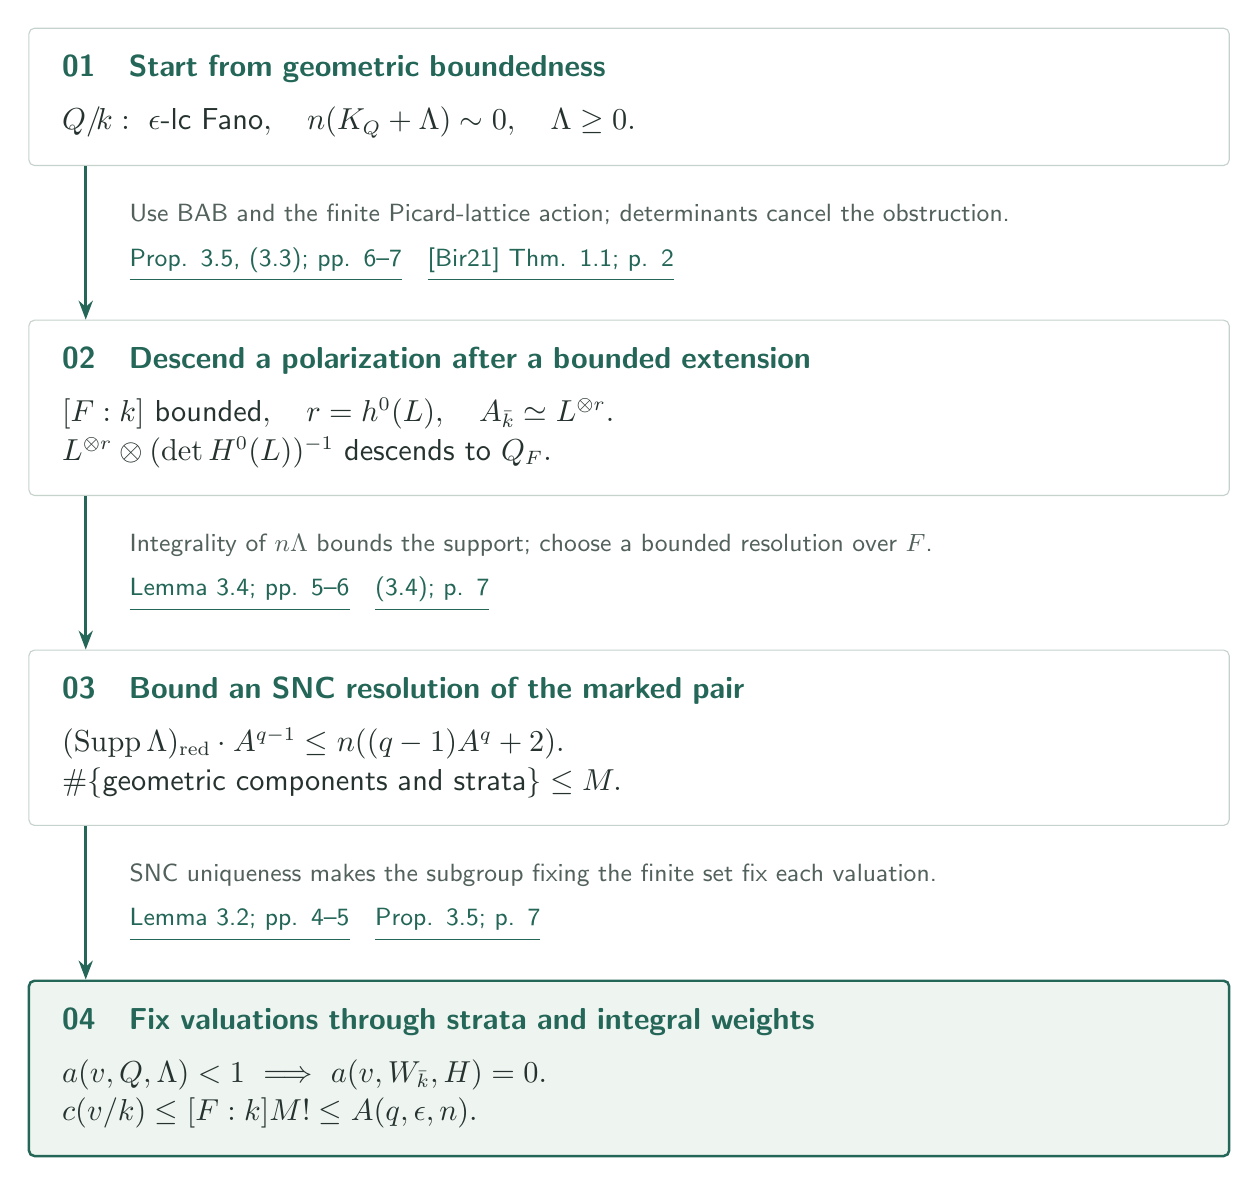
\begin{tikzpicture}
\node[card] (n0) {\heading{01}{幾何学的有界性から出発}{Start from geometric boundedness}$Q/\!k:\ \epsilon\text{-lc Fano},\quad n(K_Q+\Lambda)\sim0,\quad \Lambda\ge0.$};
\node[card,below=1.95cm of n0] (n1) {\heading{02}{有界な拡大で偏極を降下}{Descend a polarization after a bounded extension}$[F:k]\text{ bounded},\quad r=h^0(L),\quad A_{\bar k}\simeq L^{\otimes r}.$\\ $L^{\otimes r}\otimes(\det H^0(L))^{-1}\text{ descends to }Q_F.$};
\flow{n0}{n1}{\Tx{BABとPicard格子の有限Galois像を使い、行列式で障害を消す。}{Use BAB and the finite Picard-lattice action; determinants cancel the obstruction.}\\[4pt]\Cite{https://github.com/openai/math/blob/adc7f1241b42e322a6451854ab7e4b4c146bf78a/preprints/Arithmetic-Stein-degree-bounds-for-log-Calabi-Yau-pairs-September-25-2026/paper.pdf}{Prop. 3.5, (3.3); pp. 6--7}\quad \Cite{https://arxiv.org/pdf/1609.05543v2}{[Bir21] Thm. 1.1; p. 2}}
\node[card,below=1.95cm of n1] (n2) {\heading{03}{境界を含むSNC解消を有界にする}{Bound an SNC resolution of the marked pair}$(\operatorname{Supp}\Lambda)_{\rm red}\cdot A^{q-1}\le n((q-1)A^q+2).$\\ $\#\{\Tx{\text{幾何学的成分とstrata}}{\text{geometric components and strata}}\}\le M.$};
\flow{n1}{n2}{\Tx{$n\Lambda$ の整性で台の次数を抑え、体上の有界解消を選ぶ。}{Integrality of $n\Lambda$ bounds the support; choose a bounded resolution over $F$.}\\[4pt]\Cite{https://github.com/openai/math/blob/adc7f1241b42e322a6451854ab7e4b4c146bf78a/preprints/Arithmetic-Stein-degree-bounds-for-log-Calabi-Yau-pairs-September-25-2026/paper.pdf}{Lemma 3.4; pp. 5--6}\quad \Cite{https://github.com/openai/math/blob/adc7f1241b42e322a6451854ab7e4b4c146bf78a/preprints/Arithmetic-Stein-degree-bounds-for-log-Calabi-Yau-pairs-September-25-2026/paper.pdf}{(3.4); p. 7}}
\node[result,below=1.95cm of n2] (n3) {\heading{04}{付値をstratumと整数重みで固定する}{Fix valuations through strata and integral weights}$a(v,Q,\Lambda)<1\ \Longrightarrow\ a(v,W_{\bar k},H)=0.$\\ $c(v/k)\le[F:k]M!\le A(q,\epsilon,n).$};
\flow{n2}{n3}{\Tx{SNC付値の一意性から、有限集合を固定する群が各付値を固定。}{SNC uniqueness makes the subgroup fixing the finite set fix each valuation.}\\[4pt]\Cite{https://github.com/openai/math/blob/adc7f1241b42e322a6451854ab7e4b4c146bf78a/preprints/Arithmetic-Stein-degree-bounds-for-log-Calabi-Yau-pairs-September-25-2026/paper.pdf}{Lemma 3.2; pp. 4--5}\quad \Cite{https://github.com/openai/math/blob/adc7f1241b42e322a6451854ab7e4b4c146bf78a/preprints/Arithmetic-Stein-degree-bounds-for-log-Calabi-Yau-pairs-September-25-2026/paper.pdf}{Prop. 3.5; p. 7}}
\end{tikzpicture}

\end{document}
